\documentclass{article}

\usepackage[portuguese]{babel}

\usepackage{amsmath, amssymb}
\usepackage{graphicx}
\usepackage{listings}
\usepackage[colorlinks=true, allcolors=blue]{hyperref}

\usepackage[section]{placeins}

\title{Relatório 01}
\author{Vinícius de Oliveira Peixoto Rodrigues (245294)}
\date{Agosto de 2022}

\begin{document}
\maketitle

\section*{Questão (d)}

\subsection*{Item 1}
A saída do programa é:

\begin{verbatim}
    1a. Leitura:
    9876543210
    9876543210
    9876543210
    9876543210
    98
    2a. Leitura:
    76543210
    9876543210
    9876543210
    9876543210
    9876
    3a. Leitura:
    543210
    9876543210
    9876543210
    9876543210
    987654
\end{verbatim}

\subsection*{Item 2}

A variável \texttt{i} é um file descriptor para o arquivo indicado pelo \texttt{argv[1]} (primeiro argumento do programa), no caso o \texttt{teste.d}; a variável \texttt{j} é um file descriptor obtido a partir da syscall \texttt{dup(int oldfd)}, de modo que \texttt{i} e \texttt{j} compartilham do mesmo status e file offset. Por isso, quando são lidos 50 bytes pelo fd \texttt{i}, na próxima chamada do \texttt{read} (onde é usado o fd \texttt{j}), é feita a leitura a partir de onde se parou no \texttt{i} (visto que ambos compartilham o mesmo file offset).

\section*{Questão (e)}

\subsection*{Itens 1 e 2}

\begin{verbatim}
> ./e teste1.e ls -s
> cat teste1.e
total 2108
  16 a
   4 a.c
  16 b1
   4 b1.c
  16 b2
   4 b2.c
  16 c
   4 c.c
  16 d
   4 d.c
  16 e
   4 e.c
   4 f.c
   4 g.c
   4 h.c
   4 teste.a
   4 teste.b
   4 teste.d
   0 teste1.e
   8 testec1.txt
1956 testec2.txt
\end{verbatim}

O programa cria um arquivo com o nome dado em \texttt{argv[1]} (primeiro argumento do programa); em seguida, duplica o file descriptor e atribui o número de fd \texttt{1} (equivalente ao \texttt{stdout}). Em seguida, fecha o descritor original e executa a syscall \texttt{execvp(char *file, char *argv[])}, passando como \texttt{file} o \texttt{argv[2]} (\texttt{ls}) e como argumentos o \texttt{\&argv[2]} (\texttt{["ls", "-s"]}).

Essencialmente, o programa faz uma redireção da saída (redireciona o output de \texttt{argv[2]} para o arquivo \texttt{argv[1]}).

\subsection*{Itens 3, 4 e 5}

\begin{verbatim}
> ls -s > teste2.e
> cat teste2.e
total 2112
  16 a
   4 a.c
  16 b1
   4 b1.c
  16 b2
   4 b2.c
  16 c
   4 c.c
  16 d
   4 d.c
  16 e
   4 e.c
   4 f.c
   4 g.c
   4 h.c
   4 teste.a
   4 teste.b
   4 teste.d
   4 teste1.e
   0 teste2.e
   8 testec1.txt
1956 testec2.txt
\end{verbatim}

O comando acima faz a mesma coisa: redireciona o output do comando \texttt{"ls -s"} para um arquivo (no caso \texttt{teste2.e}). Ele funciona da mesma forma que o programa \texttt{e.c}.

\section*{Questão (f)}

\subsection*{Item 1}
\begin{figure}[!ht]
    \begin{center}
        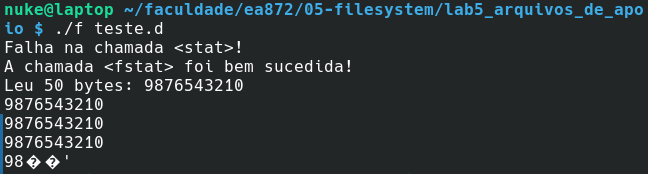
\includegraphics[width=\textwidth]{images/questao_f.png}
    \end{center}
\end{figure} 
\FloatBarrier

\subsection*{Item 2}

Porque o hard link \texttt{tmp} havia sido excluído por meio da chamada \texttt{unlink} (de modo que foi excluído o hard link em si, mas não o arquivo para o qual ele apontava).

A chamada \texttt{fstat} foi feita usando o número do file descriptor do arquivo (\texttt{argv[1]}) em si, obtido enquanto o hard link \texttt{tmp} ainda estava vivo.

\subsection*{Item 3}

O programa falhará na chamada \texttt{open("tmp", ...)}, visto que não há um arquivo (ou hard link) com esse nome.

\subsection*{Item 4}

A syscall \texttt{read} não coloca um null terminator (\texttt{'\textbackslash 0'}) 
após copiar o conteúdo do buffer, de modo que o \texttt{printf} vai ler lixo até encontrar um byte zero na pilha do programa. Para evitar isso, a forma mais simples seria escrever um \texttt{'\textbackslash 0'} 
no final do buffer:

\begin{verbatim}
    buf[i] = 0;
\end{verbatim}

\section*{Questão (g)}
\subsection*{Itens 1 e 2}

\begin{figure}[!ht]
    \begin{center}
        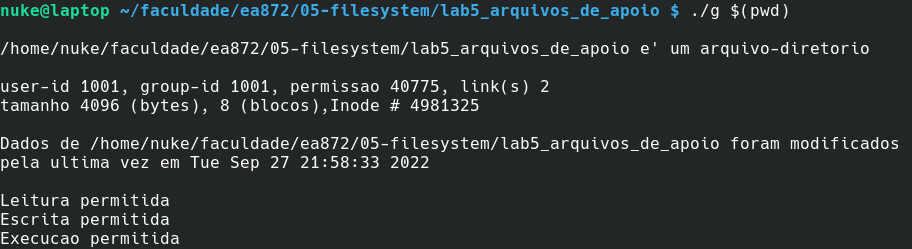
\includegraphics[width=\textwidth]{images/questao_g1.png}
    \end{center}
\end{figure} 

\begin{figure}[!ht]
    \begin{center}
        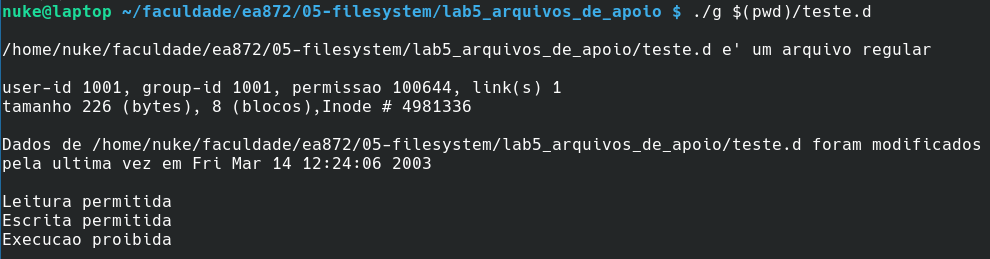
\includegraphics[width=\textwidth]{images/questao_g2.png}
    \end{center}
\end{figure} 

\begin{figure}[!ht]
    \begin{center}
        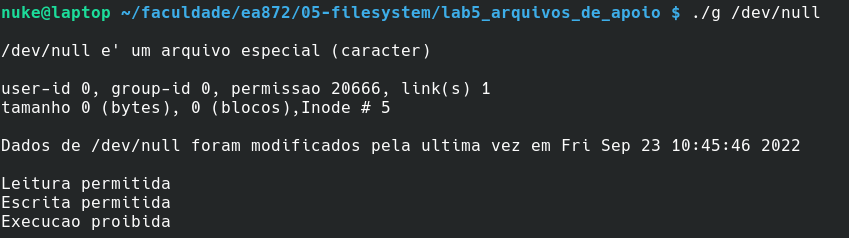
\includegraphics[width=\textwidth]{images/questao_g3.png}
    \end{center}
\end{figure} 
\FloatBarrier

O programa usa a syscall \texttt{stat} para obter os atributos de um arquivo e os imprime no console.

\section*{Questão (h)}

\end{document}

